\chapter{Introduction}

  \epigraph{Talk is cheap. Show me the code.}{Linux Torvald}

	\section{Le tracking vidéo}
	
  Le tracking d'objets à partir d'enregistrements vidéo est un problème qui a beaucoup gagné en popularité ces dernières années. Cela est dû en grande partie à son grand potentiel, aussi bien en science que pour des applications commerciales ou de sécurité. On citera par exemple le cas des voitures autonomes \cite{viswanathan2017applications} qui peuvent se conduire seul, ou bien le projet ATTOL \cite{ATTOL} de la compagnie Airbus qui permet un décollage, un atterrissage et roulage au sol entièrement automatisé reposant uniquement sur de l'analyse d'images. Une grande partie des efforts de recherche est mise sur la création d'algorithmes de reconnaissance et de tracking de piétons \cite{}, dans le but d'automatiser l'analyse des données de vidéo surveillance. Le tracking est aussi très utilisé dans le domaine du cinéma et des effets spéciaux (VFX). Que ce soit pour stabiliser les prises de vues ou bien réaliser des effets spéciaux (ex. motion capture). Dans ce cas, le tracking automatisé sur images permet de réduire les coûts et les temps de production. En science, l'utilisation du tracking automatisé, surtout en biologie et en écologie \cite{dell2014automated}, est un domaine en plein essor. Il évite de devoir marquer de manière invasive les animaux et donc de les perturber. Il permet de générer un grand nombre de données fiables, de réduire les biais, en évitant au passage une analyse manuelle longue et laborieuse.
\medbreak
  Le tracking d'objets peut être séparé en deux catégories : le Single Objet Tracking (SOT), où le but est de détecter un seul objet dans une scène plus ou moins complexe, et le Multiple Object Tracking (MOT) \cite{luo2014multiple} où il faut cette fois-ci détecter et suivre plusieurs objets. On se placera ici dans le cadre du MOT en quasi deux dimensions appliquée en grande majorité au domaine scientifique. Cela réduit grandement la difficulté du problème, en général la qualité des images est bonne, la caméra est fixe, et on peut optimiser l'éclairage pour faciliter la détection des objets. En contrepartie, la tolérance aux erreurs est faible si on veut pouvoir produire des données fiables, et donc des conclusions scientifiques robustes. Un point déterminant est la performance de l’algorithme qui doit pouvoir analyser les données dans un temps raisonnable comparé à leur débit de production, et répondre aux contraintes matérielles et techniques de l'utilisateur. La facilité d'installation et d'utilisation du logiciel qui intègre l’algorithme ne doit pas être négligée. Les utilisateurs amenés à utiliser ces logiciels ne sont en général pas des experts du domaine informatique et d'analyse d'images et le logiciel doit être facilement installable et utilisable par tous.
\medbreak
  On verra d'abord en quoi le tracking est un problème complexe et, comment on peut réduire ou contourner cette complexité. En présentera ensuite une liste non exhaustive des logiciels existants en matière de tracking appliqué aux domaines scientifiques. Enfin on verra en quoi l'approche de FastTrack, le logiciel que nous avons créé pour résoudre le problème du tracking, est différente et dans quels cas elle peut être utile.


	\section{Le tracking, un problème compliqué}
  Le tracking d'objets à partir d'images repose sur trois étapes clés : l'acquisition des images qui en fonction des paramètres d'acquisition conditionnera la difficulté du tracking et le type d'algorithme utilisable, la détection des objets qui consiste à séparer les objets du fond, et enfin l'assignation des objets d'une image sur l'autre permettant de conserver leurs identités. La tracking d'objet est en général un problème de traitement d'images complexe \cite{dell2014automated}. D'une part en fonction des objets étudiés, par exemple en biologie les animaux sont des objets grandement déformables ce qui complique la détection. D'autre part la scène peut être complexe, avec des objets disparaissant derrière des éléments du décor, se superposant (phénomène dit d'occlusion) ou entrant et sortant du champ de vue en permanence, complique l'étape d'association.
\medbreak
  
  Les problèmes de détection d'objets peuvent en général être contournés par la conception de l'expérience quand cela est possible. Un point de vue fixe et une optimisation de l'éclairage permettent en général une simple détection par soustraction d'une image de fond (sans objets) et application d'un seuil. Pour les cas plus compliqués, une grande variété algorithme est disponible \cite{yilmaz2006object} et applicable suivant la qualité des images. Les plus courants sont la détection de points d’intérêt de l'objet, invariant par rapport au point de vue et de l'illumination, cette technique nécessite une bonne qualité d'image. La segmentation permet de séparer l'image par zone de similarités et donc de détecter les objets d’intérêts, de nombreux algorithmes et approches existent pour segmenter une image. Le machine learning peut aussi être appliqué pour la détection des objets \cite{zhao2019object}.
\medbreak
  Deux grandes classes d’algorithmes se distinguent pour mitiger les problèmes d'association. La première classe d’algorithme utilise les quantités cinématiques de l'objet, comme sa vitesse ou sa position \cite{rodriguez2017toxid, qian2016effective}, pour prédire ou retrouver à postériori la position de l'objet et ainsi garder son identité. Le taux d'erreurs de cette méthode reste constant quand on augmente le nombre d'individus, elle est en général rapide et cela en fait donc un bon candidat pour les applications de tracking en temps réel. L’inconvénient majeur de cette approche vient du phénomène de propagation des erreurs. Si l'algorithme fait une erreur dans l'assignation, alors il n'a aucun moyen de corriger l'erreur à l'étape suivante et elle se propage jusqu'à la fin de l'analyse.
  Une deuxième classe d’algorithme est basée sur la reconnaissance de points d'intérêts de l'objet, permettant ainsi de créer une "empreinte digitale" unique à chaque objet, en utilisant soit une méthode classique \cite{perez2014idtracker, bai2018automatic}, soit du machine learning \cite{mathis2018deeplabcut, romero2019idtracker}. Cela permet de solutionner le problème de la propagation des erreurs d'assignation et également de suivre des objets dans le temps, par exemple un animal d'un jour d'expérience sur l'autre, ce qui peut être très utile notamment pour certaines applications d'étude du comportement. Cette méthode nécessite une image de qualité suffisante pour détecter des marqueurs représentatifs de l'objet. En général, elle demande aussi plus de ressources matérielles, donc une analyse qui ne peut pas être faite en temps réel. Mais la principale limitation est le nombre d'objets qu'elle peut suivre, il est actuellement limité à une dizaine d'objets par image avant que la performance  des algorithmes se dégradent significativement avec les méthodes classiques. L'approche par machine learning permet d'augmenter le nombre d'objets au prix d'un temps de calcul long et la nécessité d'avoir recours à des machines très performantes.
	
	\section{Les logiciels existants}
  De nombreux logiciels de tracking existent déjà, on fera ici une liste non exhaustive des plus populaires en les séparant en deux catégories : les logiciels open-sources et les logiciels propriétaires.

  \subsection{Les logiciels propriétaires}
  Les logiciels propriétaires présentés ici sont closed-sources, l'utilisateur ne peut pas modifier le code pour adapter le logiciel à son projet. En contrepartie ils ne nécessitent aucune connaissance en informatique et bénéficie d'un service d'assistance. Ils sont une bonne alternative à d'autres options parfois difficiles à mettre en place mais leurs prix élevés peuvent être un frein pour certain laboratoire.
  
  \paragraph{EthoVision XT}
  EthoVision XT est un logiciel développé par la société Noldus. Il accompagne l'utilisateur de l'acquisition des images grâce à un système de templates d'expériences, jusqu'à l'analyse des données avec un module permettant de visualiser les quantités intéressantes. Le logiciel est très complet et très largement utilisé. Il est plutôt spécialisé dans le domaine des neurosciences comportementales. Il inclut des modules pour les expériences typiques comme un "module d'interaction social pour rats", "water maze" etc... Il permet aussi d'effectuer le tracking en direct, ce qui permet de ne pas à avoir à enregistrer les images.
\medbreak
  EthoVision XT est un logiciel mature, un grand nombre de modules est disponible ainsi qu'un système permettant de créer soit-même des templates d'expériences. Le plus gros inconvénient est que l'utilisateur ne peut pas modifier le logiciel ou contrôler comment le tracking y est effectué. Le prix peut-être une barrière pour certains utilisateurs, le logiciel coûtant au minimum 5 850 USD sans module. Il est compatible avec Windows uniquement.
  
  \paragraph{Any-maze}
  Any-maze est un logiciel développé par la société Stoelting Co. Any-maze est spécialisé dans l'analyse des expériences de neuroscience comportementale. Il intègre directement des outils pour les tests les plus connus tel que le "forced swim test" ou le "fear conditionning test" permettant une analyse entièrement automatique de ces expériences. Il peut faire du tracking en temps réel ou depuis des vidéos déjà enregistrées.
\medbreak
  Any-maze est très complet dans l'analyse des expériences typiques de comportement et peut être acheté avec le dispositif expérimental déjà optimisé et calibré pour le logiciel. La suite Any-maze se décompose en trois logiciels, la partie tracking est disponible au prix de 6 495 USD ou 1 500 USD l'année. Le logiciel est disponible pour Windows uniquement. 

  \subsection{Les logiciels open-sources}
  Les logiciels open-sources permettent à l'utilisateur de modifier et distribuer le logiciel. C'est la meilleure alternative aux logiciels commerciaux. En contrepartie aucune assistance n'est fournie, le développement collaboratif de certains logiciels (par exemple sur Github) permet de signaler des bugs et de participer à leur correction et donc d'améliorer le logiciel.

  \paragraph{idTracker} idTracker \cite{perez2014idtracker} est une bibliothèque MATLAB qui permet de tracker plusieurs objets. Il est basé sur l'extraction d'une "empreinte digitale" pour chaque objet, et donc une détection fiable sans propagation d'erreurs. L'avantage d'idTracker est qu'il peut reconnaitre un objet sur plusieurs vidéo et après une relativement longue période de temps, ce qui peut être utile pour suivre le comportement d'individus sur plusieurs séries d'expériences s'étalant dans le temps. IdTracker est cependant limité par le nombre d'objets qu'il peut tracker, actuellement une vingtaine, dû à la longueur des vidéos nécessaire à l'extraction optimale de "l'empreinte digitale" de chaque objet, qui peut aller jusqu'à 30 minutes minimum pour une grande densité d'objet. La qualité requise des images est un facteur important et doit au moins être de 150 pixels par animales. Le temps de calcul est relativement long, de l'ordre de 0.5 à 2 secondes par image et nécessite une grande quantité de RAM. L'installation d'idTracker peut se faire sans avoir besoin d'acheter MATLAB grâce au Matlab Run Time Compiler mais uniquement sous Windows. Il est par conséquent nécessaire d'acheter une licence MATLAB pour les autres plateformes, et d'avoir une connaissance minimale du langage pour mettre en place idTracker.

  \paragraph{ToxTrack}
  ToxTrack \cite{rodriguez2018toxtrac} est un logiciel qui implémente dans une interface graphique l'algorithme ToxId \cite{rodriguez2017toxid}. L’algorithme extrait les objets du fond en appliquant un seuil. Les morceaux de trajectoire entre chaque occlusion sont ensuite divisés en trajectoires courtes et trajectoire longues basé sur une durée seuil définis par l'utilisateur. Un groupe de trajectoires longues où tous les individus sont observés en même temps est alors extrait, dans ce cas là l'assignation est fait grâce à l'algorithme Hongrois. Les trajectoires courtes sont ensuite assignées à l'objet correspondant par corrélation entre une matrice d'identification des trajectoires.
  Les auteurs rapportent que ToxId est aussi performant que les logiciels déjà existants, très rapide, il est possible de tracker les objets en temps réel. Un désavantage que l'on peut constater dans cet algorithme est qu'il ne marche seulement que pour un nombre constant d'animaux. L'initialisation de l'algorithme nécessite d'avoir à un instant $t$ l'ensemble des objets à tracker simultanément détectable pendant un temps $t+dt$ défini par l'utilisateur. Le gui inclus des outils permettant de définir des zones d’intérêt ainsi qu'une analyse statistique des données recueillies. On constate que la matrice de corrélation de trajectoire ne permet pas une reconnaissance de l'objet et que les erreurs avec cette méthode sont propagatives. Le logiciel est disponible pour Windows et compilable pour les autres systèmes.

  \paragraph{DeepLabCut}
  DeepLabCut \cite{mathis2018deeplabcut} est un framework qui permet de résoudre le problème dit de "pose estimation" qui consiste à retrouver un objet et sa position, ou une partie d'objet, dans une image. Il peut directement s'apparenter au problème du SOT si les objets à tracker sont différents, exemple une oreille droite et un nez de souris, qui pourront ensuite être retrouvé sur chaque image puis associées dans le cas où il n'y a qu'une seule souris. Dans le cas de plusieurs objets similaires à retrouver et associer d'une image sur l'autre (MOT), il faudra combiner cette détection avec une association pour obtenir le tracking. Même si DeepLabCut répond à un problème légèrement différent, il peut, par sa conception être couplé à un algorithme d'association externe pour en faire un logiciel de tracking.
\medbreak
  DeepLabCut est directement basé sur l'algorithme de détection de feature du framework DeeperCut \cite{insafutdinov2016deepercut}, spécialisé dans la détection des mouvements du corps humain. Les auteurs de DeepLabCut ont étudié les performances de cet algorithme appliqué au domaine des neurosciences comportementales, comme la détection du museau d'une souris, ou des pattes d'une drosophile, et ont ajouté des outils permettant de facilement entrainer l’algorithme et de tester sa robustesse. Il tire parti du deep learning pour résoudre le problème de "pose estimation". Pour rappel, le deep learning est un type d'algorithme de machine learning qui consiste à entraîner un réseau de neurones possédant plusieurs couches. Ce réseau est constitué de plusieurs ResNets (residual neural network) qui ont été pré-entrainés sur la base de données ImageNet. Des couches de déconvolution sont placées en sortie des ResNets et permettent d'obtenir la probabilité de présence de l'objet dans l'image. Le réseau est ensuite finement ajusté en l’entrainant sur des images où sont annotées les parties qui doivent être détectées. Les auteurs ont ainsi montré qu'on peut obtenir une performance au moins aussi bonne que celle d'une détection par un être humain avec très peu de données d’entrainements, de l'ordre de 200 images.
\medbreak
  DeepLabCut, comme indiqué précédemment, est une framework, et malgré une très bonne documentation \cite{nath2019using}, il peut être difficile à mettre en place pour un utilisateur possédant peu de compétence en informatique. Le processus d'installation durant de 10 à 60 minutes et nécessitant l'installation d'un GPU et des drivers associés pour tirer au mieux parti du logiciel. De plus, l'algorithme demande beaucoup de puissance de calcul et un GPU (NVIDIA GForce 1080 8GB au moins) est fortement conseillé. Pour donner un ordre d'idée, des images de 682x540 pixels, analysées avec un GPU de dernière génération, permet d'attendre une vitesse d'analyse de 30 images par seconde, sans GPU ce temps peut être multiplié par un facteur 10 où 100 \cite{mathis2018inference}.
\medbreak
  On voit donc que DeepLabCut présente un grand intérêt pour retrouver dans une image des objets avec une grande précision. Il s'adresse plus particulièrement aux neurosciences comportementales où il permet de suivre des mouvements complexes (ex. doigt de la main chez une souris). Il ne conviendra pas aux utilisateurs avec peu de connaissances en informatique s’intéressant à des problèmes plus larges et ayant une grande quantité de données à traiter.

  \paragraph{idTracker.ai}
  IdTracker.ai \cite{romero2019idtracker} est un framework qui permet de tracker des animaux (de l'ordre d'une centaine) avec une précision quasi parfaite. IdTracker.ai tire parti du deep learning pour réaliser le tracking. Dans une première étape, chaque objet est segmenté en appliquant un seuil. Un réseau convolutionnel classe ensuite chaque blob détecté comme contenant un objet seul, ou contenant plusieurs objets. Un autre réseau convolutionnel permet ensuite de trouver l'identité de chaque individu tout au long du film. Pour fonctionner, ce système nécessite assez de données pour pouvoir entrainer le réseau à reconnaitre chaque individu. Les auteurs ont trouvé qu'un tracking robuste peut être obtenu avec seulement 30 images isolées de chaque individu comme base, il faut donc prévoir au minimum des vidéos de 500 images pour une dizaine d'individus avec un minimum de 25 fps. Une résolution de 300 pixels par animale est recommandée pour avoir une bonne précision de tracking. Un facteur limitant d'idTracker.ai est qu'il demande beaucoup de temps de calcul et beaucoup de RAM, les auteurs rapportent une durée du vingtaines de minutes pour 8 zebrafish et de l'ordre de 6 heures pour 100 zebrafish sur environ 2000 images hautes définitions. Même si un gui est disponible pour aider l'utilisateur, des connaissances de base en informatique et en programmation sont nécessaires, tout comme un matériel adapté, l'utilisation d'un GPU est fortement recommandé. Il est recommandé à des utilisateurs souhaitant un tracking parfait, entièrement automatisé depuis des images de grandes qualités et des films assez long possédant une machine puissante et sans contrainte de temps.

	\section{FastTrack : une approche différente}
  On a vu précédemment les logiciels existant ainsi que les différents paradigmes du tracking appliqué aux sciences. On voit qu'une approche rapide, nécessitant peu de puissance de calcul, et généraliste (pouvant s'appliquer à différents systèmes, nombre d'objets variable, etc...) est manquante.
	Pour combler ce vide, nous avons conçu un logiciel nommé FastTrack. Ce logiciel contient deux parties distinctes :
	\begin{itemize}
		\item Une interface où sont implémentés les procédures standards d'analyse d'images permettant la détection des objets, et un algorithme de tracking qui permet de conserver l'identité des objets d'une image sur l'autre, rapide et avec un faible taux d'erreur.
		\item Une interface ergonomique permettant la vérification et éventuellement la correction manuelle de toutes erreurs ayant pu être commise par l’algorithme de tracking.
	\end{itemize}
	On remarquera ici la différence d'approche entre FastTrack et les logiciels existant. Au lieu de développer un système nécessitant une grande puissance de calcul, longue mais apportant des résultats entièrement automatisés et d'une grande fiabilité, FastTrack implémente une méthode rapide et facile à paramétrer, très généraliste. La correction des erreurs restantes est laissé à la charge de l'utilisateur mais peut-être effectué nativement dans le logiciel, l'interface ergonomique permettant une correction rapide et efficace. 
	Cette solution présente plusieurs avantages, le premier étant qu'elle ne nécessite aucune connaissance en programmation, n'importe quel utilisateur peut réaliser une analyse parfaite en très peu de temps. De plus, on a pu montrer que le travail de post-traitement peut être estimé a priori par une analyse des paramètres géométriques et dynamiques du système étudié ce qui permet à l'utilisateur de savoir si le logiciel est adapté à ses besoins. Pour beaucoup de systèmes étudiés, le post-traitement se résume à une rapide vérification. Dans certains cas, si le nombre d'occlusions est trop importantes et qu'une précision de tracking parfaite est nécessaire sans vouloir avoir recours à une correction manuelle, une autre solution doit être envisagée.
\medbreak
	FastTrack est distribué sous une licence open-source et implémenté de manière modulaire et entièrement documenté. Chaque utilisateur peut ainsi modifier le logiciel à sa convenance ou y contribuer. L'algorithme de tracking est découplé de l'interface de détection et de correction se qui rend extrêmement facile l'intégration de FastTrack dans un projet déjà existant. Le logiciel est facilement installable en moins de 5 minutes et est compatible Linux, MacOs et Windows, il peut fonctionner sur des configurations modestes et des Single Board Computer (SBC) tel que le Raspberry Pi.


\chapter{Conception et réalisation}

    \epigraph{Testing can only prove the presence of bugs, not their absence.}{Edsger W. Dijkstra}

	\section{Outils utilisés}
	
	Le choix des outils et bibliothèques utilisés dans la conception d'un logiciel est primordial et plusieurs facteurs de sélection doivent être pris en compte.
	Le premier critère à considérer est celui de la licence, j'ai fait le choix de mettre le logiciel FastTrack sous licence libre (GPL3) ce qui implique que le langage utilisé ainsi que les bibliothèques soient elles aussi sous des licences compatibles (MIT, GPL, etc...). Le choix d'une licence open-source est évident dans le cas d'un logiciel scientifique, l'utilisateur pouvant alors vérifier comment le logiciel fonctionne, le modifier pour l'adapter à ses besoins ainsi que le partager.
	Le deuxième critère est de bien choisir les bibliothèques utilisées en envisageant le futur du logiciel de manière à ne pas avoir à changer de bibliothèques si ses capacités s'avèrent insuffisante à mesure que le logiciel évolue. On privilégiera les bibliothèques matures offrant un support sur le long terme.
\medbreak
	
	Dans cette perspective, FastTrack a été implémenter en C++ \cite{C++} en utilisant les bibliothèques Qt \cite{Qt} et OpenCV \cite{opencv_library} respectivement pour l'interface graphique et l'analyse d'image. Les tests unitaires sont réalisés à partir de la bibliothèque Google Test.
\medbreak
	
	Le C++ est un langage informatique créer par Bjarne Stroustrup en 1985. Offrant de grandes performances, il est standardisé par l'International Organization for Standardization (ISO) et est le language de choix pour les applications d'analyse d'images ainsi que la création d'interfaces graphiques complexes.
\medbreak
	
	Qt est une bibliothèque d'interface graphique open-source créée par Haavard Nord et Eirik Chambe-Eng, tous deux physiciens, en 1991 alors qu'ils réalisaient un logiciel d'analyse d'images ultrasoniques. Très mature, possédant une vaste documentation, une très grande communauté, elle permet de réaliser des interfaces graphique pour Linux, Mac et Windows avec le même code source.
\medbreak
	
	OpenCV est une bibliothèque d'analyse d'images open-source créée par Intel en 1999. Très complète et efficace, elle est devenue la référence en matière d'analyse d'images aussi bien en recherche que pour la réalisation d'applications commerciales.
\medbreak
	
	Google test est une suite permettant d'automatiser les tests unitaires en C++, elle est notamment utilisée par OpenCV. Le but des tests unitaires est de vérifier que chaque partie du programme fonctionne comme attendu. Cette pratique présente plusieurs avantages, les principaux étant de détecter plus facilement d'éventuelles erreurs lors de l'implémentation de nouvelles fonctionnalités, et de faciliter le développement du logiciel quand celui-ci grandi en taille pour éviter toutes inclusions d'erreurs. Cette série de tests est automatiquement effectuée à chaque nouveau commit, voir section~\ref{}.
	
	\section{Implémentation}
	
	Le fonctionnement de FastTrack peut être séparé en trois parties que sont : la détection des objets, l'association des objets d'une image sur l'autre, et enfin une étape de correction.
\medbreak
	
	Chaque analyse commence par l'ouverture d'une séquence d'images, ou d'un film. L'utilisateur a le choix entre deux types d'interfaces, une interface interactive où il ne peut ouvrir qu'un seul film à la fois. Elle permet de voir en temps réel l'impact des paramètres sur les images ce qui facilite la détermination des paramètres optimaux d'analyse. Une deuxième interface permet d'ouvrir simultanément une grande quantité de films, soit en donnant un fichier de paramètres ou en sélectionnant les paramètres dans l'interface. Elle est utile quand l'utilisateur veut analyser un grand nombre de films dont il connaît déjà les paramètres optimaux d'analyse.
\medbreak
	
	Les deux interfaces peuvent être utilisées de manière complémentaire. L'utilisateur peut trouver les paramètres optimaux avec l'interface interactive et ensuite automatiser l'analyse d'un grand nombre de films en les ajoutant par lots dans le logiciel.
	
	\begin{figure}[h]
    \centering
    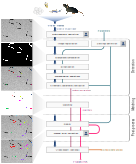
\includegraphics[width=0.75\textwidth]{part_1/assets/Figure_1.png}    
    \caption{\textbf{FastTrack flux de traitement.} Il se divise en trois parties distinctes : la détection, l'association et le post-traitement.}
    \label{part_1:fig_1}
    \end{figure}
	
	
		\subsection{Détection}
		
		L'étape de détection a pour but d'extraire les paramètres cinématiques de chaque objet qui seront ensuite utilisé dans l'étape d'association. FastTrack inclut une collection de filtres d'analyse d'images permettant à l'utilisateur d'optimiser la détection des objets sans avoir à recourir à un logiciel externe.
		
		
		\paragraph{Calcul du fond}
		Chaque analyse commence par calculer une image de fond. Si l'utilisateur possède déjà une image de fond préalablement enregistrée, il peut directement l'ouvrir dans le logiciel. Sinon trois méthodes de calcul sont possibles :
		\begin{itemize}
			\item Projection du maximum d'intensité.
			\item Projection du minimum d'intensité.
			\item Projection de la moyenne d'intensité.		
		\end{itemize}
		Les trois méthodes reposent sur le même principe. L'utilisateur choisit $n$ images dans la séquence, le logiciel va projeter dans la direction perpendiculaire à l'image (le long de la composante temporelle) soit le maximum, soit le minimum ou bien la moyenne de la séquence. En pratique, on projettera le maximum (resp. minimum) si les objets sont plus foncés (resp. clairs) que le fond de manière à faire disparaître les objets et ainsi obtenir le fond. L'utilisateur peut effectuer une registration de chaque image avant projection de manière à corriger un éventuel mouvement de la caméra.
		
		
		\paragraph{Registration}
		L'utilisateur peut choisir d'effectuer une registration des images, trois méthodes sont proposées dans le logiciel. Chaque méthode est implémentée de manière pyramidale, c’est-à-dire que la registration est d'abord effectuée sur une image dégradée pour corriger de manière grossière le déplacement, puis la correction est affinée en augmentant la qualité de l'image jusqu'à arriver à l'image originelle. Cela permet d'accélérer le processus, la registration étant souvent un procédé relativement coûteux en temps de calcul.
\medbreak
		
		La première méthode proposée est la corrélation de phase. Elle permet de corriger les mouvements de translation entre deux images en utilisant le théorème de Fourier dans le domaine fréquentiel. Cette méthode est très rapide mais reste limité à de petits mouvements de translation uniquement.
\medbreak
		
		La deuxième méthode proposées est la méthode Enhanced Correlation Coefficient (ECC). Dans FastTrack, elle est restreinte à corriger les mouvements de translation et de rotation uniquement. Elle consiste à utiliser le coefficient de corrélation comme mesure pour trouver la meilleure transformation entre deux images. Cette méthode a pour avantage d'être relativement rapide, le problème d'optimisation non linéaire pouvant être résolue de manière linéaire. Elle est performante pour des images bruités et ayant des distorsions photométrique (contraste, luminosité).
\medbreak
		
		La troisième méthode est une méthode basée sur le repérage de points clefs. Elle permet de corriger les mouvements et les déformations (homographie). Les points clés (environ 500) sont automatiquement déterminés sur deux images grâce à l'algorithme ORB \cite{}. Ces points sont ensuite associés deux à deux en utilisant l’algorithme RANSAC \cite{} permettant de trouver la meilleure transformation entre les deux images. Cette méthode, plus précise nécessite une qualité d'image suffisante pour pouvoir discerner des points clefs.
		
	\begin{figure}[h]
    \centering
    \includegraphics[width=1\textwidth]{part_1/assets/Figure_2.png}    
    \caption{\textbf{Registrations.} Deux films avec une dérive sévère sont utilisés comme référence (DRO\_001 en hautn ULT\_001 en bas). (\textbf{A}) Comparaison entre une image (magenta) avec la première image (vert), avec agrandissement des détails en insert. (\textbf{B}) Déviation moyenne carrée (RMSD) de l'intensité des pixels avant et après registration, moyennée sur toutes les images et normalisée par la RMSD sans registration pour les trois méthodes. Barres d'erreur : déviation standard. (\textbf{C}) Temps moyen relatif pour les trois méthodes (unités arbitraires). Barres d'erreur : déviation standard.}
    \label{part_1:fig_2}
    \end{figure}
		
		
		\paragraph{Binarisation}
		Chaque image est ensuite binarisée  en y soustrayant l'image de fond puis en définissant une valeur seuil. Dans le mode interactif, l'utilisateur peut voir l'impact des paramètres sur l'image ce qui permet d'ajuster facilement le seuil de binarisation. Le logiciel détecte également si le fond est plus foncé (resp. clair) que les objets permettant d'avoir à la fin de cette opération une image binaire  où les pixels appartenant à l’objet sont égaux à 1 et les pixels appartenant au fond sont égaux à 0.
		
		
		\paragraph{Opération morphologique}
		Un ensemble d'opérations morphologiques (dilatation, érosion, ouverture, etc...) peut-être effectuées sur l'image binaire pour améliorer la détection et éliminer d'éventuels artefacts. Différentes formes et tailles de noyaux sont disponibles.
		
		
		\paragraph{ROI}
		L'utilisateur peut sélectionner une région d’intérêt et exclure le reste de l'image de l'analyse. Cela permet d'accélérer le processus d'analyse et d'éviter la détection d’objets parasites. En mode interactif, cette ROI peut être dessiné directement sur l'image.
		
		
		\paragraph{Tri}
		Pour exclure les objets trop petits correspondant à du bruit ou trop gros, par exemple deux objets superposés, l’utilisateur doit sélectionner deux tailles caractéristiques. En mode interactif, les objets sont coloriés soit en rouge, soit en vert suivant si leur taille appartient à la gamme de tailles sélectionnée.
		
		\paragraph{Extraction des paramètres cinématiques}
		Sur la base des images binaires, le logiciel va détecter le contour de chaque objet \cite{}. Une étape importante de toute procédure de tracking est l'extraction des paramètres qui serviront dans l'étape d'association. C'est en général dans le choix de ses quantités que les algorithmes de tracking diffèrent pour se spécialiser à un type d'objet donné. Dans FastTrack, les paramètres extraient sont la position du centre de masse ainsi que l'orientation de l’objet, ses quantités sont rapidement calculées et assez généralistes pour s'adapter à une grande diversité d'objets.
\medbreak
		
		Pour faire cela, FastTrack calcule l'ellipse équivalente de l'objet à partir des moments d'ordre deux de l'image binaire. Cette procédure est accélérée en utilisant directement le contour grâce à la formule de Green \cite{}. L'orientation de l'objet est donnée par l'axe majeur de l'ellipse équivalente. Sa direction est déterminée en projetant chaque pixel de l'objet sur l'axe majeur de l'ellipse. On calcule ensuite la skewness de la distribution des distances des points projetés par rapport au centre de masse. Le signe de la skewness est un indicateur robuste de l’asymétrie de l'objet par rapport à son axe majeur à partir de laquelle on peut déterminer la direction de l'objet.
\medbreak
		
		Pour les objets déformables, la direction calculer précédemment peut être différente de la direction de déplacement. Par exemple dans le cas du poisson zèbre, celui-ci déforme son corps de manière périodique pour se déplacer, seul la tête est dirigée dans la même direction que le mouvement. C'est pourquoi on décompose l'objet en deux ellipses équivalentes, l'utilisateur peut alors choisir quelle ellipse représente le mieux la direction de déplacement.
		
		
		\subsection{Association}
		
		L'étape d'association a pour but de conserver l'identité des objets d'une image sur l'autre. Pour se faire, FastTrack utilise une méthode dérivée de \cite{}, qui tire parti du fait que la position et la direction de chaque objet change très peu d'une image sur l'autre.
		Pour chaque pair d'objet (i,j) appartenant à deux images successives, deux coûts sont calculés.
		Le coût "dur" calculé comme suit :
        $$
        \left\{
        	\begin{array}{ll}
        		h_{i,j} = 1 & \mbox{si } r_{i,j} < h_{d} \\
        		h_{i,j} = \inf & \mbox{sinon }
        	\end{array}
        \right.       
        $$
        avec $r_{i,d}$ la distance entre les objets i et j, $h_{d}$ un seuil qui représente la distance maximale de déplacement autorisée entre deux images successives.
		Le coût "mou" calculé comme suit:
		$$
        c_{i,j} = \frac{r_{i,j}}{s_d} + \frac{\delta\alpha_{i,j}}{s_{\alpha}}		
		$$
		où $\delta\alpha_{i,j}$ est la valeur absolue de la différence angulaire entre les directions de i et j, $s_{d}$ et $s_{\alpha}$ sont des coefficients de normalisation qui représente un déplacement et une réorientation typique du système étudié entre deux images successives.
		Ces deux coûts sont ensuite multipliés élément par élément pour donner la matrice suivant :
		$$
        C_{i,j} = \left\{
        	\begin{array}{ll}
        		c_{i,j} & \mbox{si } r_{i,j} < h_{d} \\
        		\inf & \mbox{sinon }
        	\end{array}
        \right.       
        $$
		La matrice de coup peut être rectangulaire si le nombre d'objets n'est pas constant comme lors d'occlusion ou d'ajout d'objets. Un paramètre de mémoire peut être sélectionné de manière à ne plus pouvoir assigner les objets si ceux-ci ont disparu depuis plus de $n$ images.
		La meilleure association possible est celle dont la somme des coûts est minimale. Ce problème est appelé "the rectangular assignement problem" et peut être résolu de manière exacte en utilisant l’algorithme hongrois, FastTrack utilise l'implémentation Kuhn-Munkres en C++ pour résoudre rapidement ce problème.
		
		\subsection{Post-traitement}
		
		\paragraph{Correction manuelle}
		FastTrack intègre un outil de correction manuel du tracking. Une fois l'analyse terminée, le résultat peut être affiché dans une interface ergonomique créée à cet effet. L'utilisateur peut rejouer le film en y superposant les résultats de l'analyse, il peut sélectionner un objet pour en consulter les paramètres (aire, contour, identité, etc...). L'utilisateur peut aussi directement corriger les erreurs en supprimant des objets ou en échangeant l'identité des objets. Cette interface est conçue dans un souci d'ergonomie et de performance. Des raccourcis clavier ainsi qu'une sélection à la volé des objets directement en cliquant sur la vidéo permettent à l'utilisateur de rapidement vérifier et corriger les analyses. Il est aussi possible d'enregistrer, en plus des données brutes d'analyse, un film avec les résultats du tracking superposés.
		Cette interface de correction manuel permet de déplacer la charge de travail qui est traditionnellement placé sur le pré-traitement des données, vers le post-traitement. Le logiciel reste alors général et peut s'adapter à une grande diversité d'objets et reste performant grâce à une interface spécialement pensée pour réduire le temps de post-traitement.
		
		\paragraph{Analyse}
		L'analyse statistique des données n'est pas implémenté dans FastTrack. Après chaque analyse, le logiciel génère un dossier contenant les résultats. Le fichier principal est nommé tracking.txt et il contient les données brutes de l'analyse avec une image et un objet par ligne. Ce format est compatible avec tous les logiciels d'analyse les plus utilisés (R, Python, MATLAB), des exemples sont disponibles dans la documentation.
		
	\section{Déploiement}
		\subsection{CI/CD}
		Le déploiement est une partie à ne pas négliger dans la conception d'un logiciel et deux aspects sont tout particulièrement important à considérer. Du point de vue de l'utilisateur, le logiciel doit pouvoir être installé facilement sur les plateformes supportées. Du point de vue du mainteneur, la partie de déploiement doit être facilement réalisable et reproductible de manière à pouvoir intégrer rapidement les correctifs et nouvelles fonctionnalités développées. C'est dans cette optique que FastTrack suit la philosophie CI/CD \cite{shahin2017continuous}\cite{wikstrom2019benefits} en tirant parti du nouveau système GitHub Actions.
\medbreak
		
		L'intégration continue (CI) est un ensemble de pratiques qui a pour but d'intégrer rapidement les changements au projet de manière automatisée. Elle est couplée avec une automatisation des tests unitaires. FastTrack tire parti du système CI/CD de GitHub nommé Actions, à chaque nouveau changement (commit\footnote{Action d'envoyer la liste de modifications effectuées dans le système de gestion de version}) ou nouvelle collaboration (pull-request \footnote{Action de demander l'ajout de modifications effectuer dans une branche au projet}), une série de tests est automatiquement déclenchée. Ces tests vont vérifier le bon fonctionnement de l'algorithme de tracking ainsi que le formatage du code source. Seul les changements qui passent les tests peuvent être intégrés au projet ce qui garantie la reproductibilité des analyses ainsi que la cohérence du code source et de la documentation.
\medbreak
		
		La livraison continue (CD) quant à elle automatise la livraison du logiciel dans sa forme finale. Elle permet d'intégrer rapidement les changements au logiciel sans avoir à le faire manuellement pour chaque plateforme supportée. Dans le cas de FastTrack, le CD est implémenté grâce à GitHub Actions et une nouvelle version du logiciel est compilée pour Linux, MacOs et Windows à chaque nouveau commit qui est intégré à la branche principale. Des versions stables du logiciel sont quant à elles compilées à chaque palier de développement. Ce système est un gain de temps majeur pour un logiciel multi-plateformes comme FastTrack, et il permet à l'utilisateur de toujours disposer des derniers correctifs et des dernières fonctionnalités.
\medbreak
		
		FastTrack supporte nativement les trois plateformes majoritairement utilisées : les systèmes Linux avec une AppImage qui supportent toutes les distributions et un PPA pour Ubuntu uniquement, Windows avec un installateur, MacOS avec une App. La dernière version stable peut-être téléchargée sur le site web \url{http://www.fasttrack.sh}, la dernière version CD sur \url{https://github.com/bgallois/FastTrack/releases}. La procédure pour compiler soit même le logiciel est disponible dans la documentation du développeur pour les autres plateformes.
		
		\subsection{Documentation}
		Une documentation extensive est disponible, elle se sépare en deux parties : une à l'usage des utilisateurs et une autre à l'usage des développeurs.
		
		\paragraph{Utilisateur} La documentation utilisateur est disponible à l'adresse \url{https://www.fasttrack.sh/UserManual/docs/intro.html}. Cette documentation est mise en forme à partir du logiciel Docusaurus et les utilisateurs peuvent y contribuer \url{https://github.com/bgallois/FastTrack/}. Elle regroupe l'ensemble des informations nécessaires à l'utilisation du logiciel ainsi que des vidéos d'explication pour aider à prendre le logiciel en mains.
		
		\paragraph{Développer} La documentation du développeur est disponible à l'adresse \url{https://www.fasttrack.sh/API/index.html}. Elle est automatiquement générée grâce au logiciel Doxygen à partir de la documentation présente dans le code source de FastTrack. Elle regroupe l'ensemble des informations nécessaires aux développeurs voulant modifier ou contribuer à FastTrack.

		
\chapter{Base de données de films}
    
    Pour démontrer que FastTrack peut être utilisé pour analyser des films provenant d'une grande diversité de systèmes, nous avons compilé une base de données de films nommée $TD^2$. Cette banque de films peut être téléchargée à l'adresse \url{https://data.ljp.upmc.fr/datasets/TD2/}. Les films proviennent soit de données déjà publiées dans la littérature, soit ils nous ont été fourni par les auteurs eux-mêmes sous licence CC-BY-NC-SA. Chaque film est identifié par un code à 3 lettres définissant le système (ex. ACT : active matter, ZFA : zebrafish adult, etc...) et 3 chiffres pour indexer les films provenant d'un système identique. $TD^2$ regroupe actuellement 41 films comprenant différents types d'objets de nature et de taille très différentes : 7 espèces d'animaux allant du poisson à la mouche, des cellules, des particules actives, des gouttes microfluidiques ainsi que des objets macroscopiques tel des joueurs d'ultimate ou des voitures. Une vidéo donnant un rapide aperçut de tous les systèmes utilisés est disponible à l'adresse suivante \url{http://www.fasttrack.sh/images/illustrations/mockups/trackingExample.webm}.
\medbreak
    Un autre aspect important à considérer est le nombre d'objets par film ainsi que leurs éventuelles apparitions, disparitions et chevauchements. Dans 22 films sur 41, le nombre d'objets est variable et des objets sortent ou rentrent dans le champ de la caméra durant l'enregistrement. Dans 19 films sur 41, des objets peuvent se chevaucher créant un phénomène d'occlusion que le logiciel doit gérer pour conserver l'identité des objets.

	\begin{figure}[h]
    \centering
    \includegraphics[width=1\textwidth]{part_1/assets/Figure_td2.png}    
    \caption{\textbf{$TD^2$.}}
    \label{part_1:fig_5}
    \end{figure}


\chapter{Résultats}

	\section{Analyse de la base de données}

  Analyser des films provenant de systèmes aussi différents que ceux compilés dans $TD^2$ est un véritable challenge. Cela est dû en partie aux conditions d'enregistrement qui peuvent être très diverses et qui complexifient la tâche de détection des objets. Deux difficultés récurrentes sont à soulever : les variations de l'illumination (ex. réflexion dans GRA\_001, ombres dans SOC\_001) et le chevauchement des objets (ex. HXB\_001).
  Dans le cas de films provenant du milieu académique, les systèmes sont souvent conçus pour limiter ou contourner ces deux difficultés. Il est commun de trouver des films dont l'illumination est uniforme et constante. de même un confinement quasi-2D ainsi qu'un nombre d'objets restreints dans le champ de la caméra permettent de réduire le nombre d'occlusions.
  Dans $TD^2$, 23 films ont une illumination assez bonne pour être analysés directement avec FastTrack, les autres ayant dû subir un pre-traitement individuel spécifique avant de pouvoir être analysées. Deux films ayant un nombre d'occlusions extrêmement élevé ont été écartés (HXB\_001 and ZFL\_001) car ne pouvant pas être analysé avec le logiciel.
  Les 39 films restant ont pu être analysés avec FastTrack sans difficulté. L'algorithme de Kuhn-Munkres étant de complexité $O(n^3)$ le temps de calcul est en général assez rapide. Sur l'ordinateur utilisé pour l'analyse (ordinateur de bureau moderne), on observe une vitesse d'analyse pouvant aller jusqu’à 500 images/secondes. Les films les plus volumineux en taille et nombre d'images ainsi qu'en nombre d'objets n'ont pas pris plus de quelques dizaines de minutes. Chaque film a ensuite été corrigé manuellement grâce à l'outil intégré dans le logiciel.
	
	\section{Estimation de la charge de travail de correction}
	
	FastTrack est conçu pour que la phase de post-traitement soit la plus faible possible, mais cette charge de travail varie grandement suivant les films analysés. On va ici montrer que cette charge de travail peut être estimée rapidement pour un film donné. On assumera pour la suite que la détection et l'association ont déjà été réalisées.
\medbreak
	
	La méthode repose sur l'évaluation de la probabilité d'incursion $P_{inc}$. Une incursion étant définie par la sortie d'un objet de sa cellule de Voronoï, prise en $t_1$, durant un trajet entre $t_1$ et $t_2$. Le nombre d'incursions dépend de la distribution des déplacements, de la densité d'objets, de la géométrie de la cellule de Voronoï et du degré d'alignement des déplacements. On peut écrite cette probabilité :
	$$$$
	où $\rho=r\sqrt{d}$ est le déplacement réduit adimensionné, $R(\rho)$ la distribution des $\rho$ et $p_{inc}(\rho)$ la probabilité géométrique d’incursion qui ne dépend que des propriétés géométrique de la disposition des objets. On calcule $p_{inc}$ en prenant les cellules de Voronoï de tous les objets sur toutes les images, puis en déterminant la proportion des angles pour lesquels un déplacement de $\rho$ implique une incursion dans une cellule de Voronoï voisine. Intuitivement, on peut se convaincre que $p_{inc}$ va de 0 quand $\rho->\inf$, à 1 quand $\rho>>1$. La forme de cette fonction est sensible à la densité des objets, compacts (ex. ACT\_002), clairsemés (ex. PAR\_001), et à la taille globale du système quand celui-ci est restreint par des murs (ex. ZFA\_001).
\medbreak
	
	Les distributions de $\rho$ et $p_{inc}$ sont représentées figure~\ref{} pour trois films de $TD^2$ représentatifs de trois systèmes très différents. Il n'est pas nécessaire d'avoir un tracking parfait pour avoir une bonne estimation de cette valeur car les quelques erreurs possibles ont une influence marginale sur la distribution des $\rho$ donc sur $P_{inc}$.
\medbreak
	On a calculé $P_{inc}$ pour tous les films de $TD^2$ figure~\ref{}, de manière à en estimer le nombre d'incursions $n_{inc}$ :
	$$
	    n_{inc}=P_{inc}*N_{obj}
	$$
	avec $N_{obj}$ le nombre total d'objet dans le film.
	Chaque incursion ne résultant pas à une inversion de l'identité de deux objets, donc à une erreur, on gardera en tête que cette valeur représente la borne maximale possible d'erreurs. Dans $TD^2$, seulement 5 films ont $n_{inc}>1$ ce qui suggère que pour la grande majorité des films, le post-traitement se résume à un simple contrôle. Les 5 films restant sont connus pour leur difficulté à être analysé dont 2 (ACT\_003 et ACT\_004) ont nécessité le développement d'un algorithme spécifique, 2 autres (BAC\_001 et ZFA\_001) des logiciels dédiés pour être analysés.
	
	\begin{figure}[h]
    \centering
    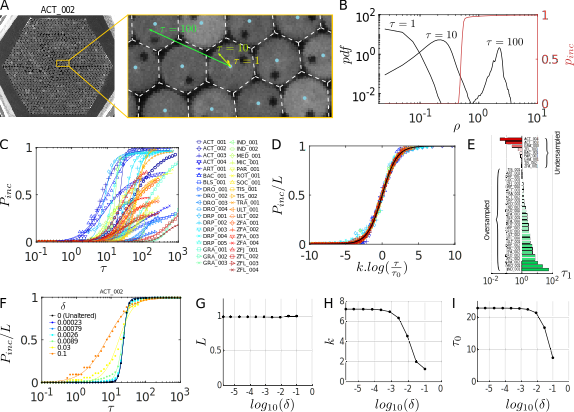
\includegraphics[width=1\textwidth]{part_1/assets/Figure_3.png}    
    \caption{\textbf{Probabilité d'incursion} (\textbf{A}) Définition des incursions : objets faisant de petits déplacements à l'intérieur de leurs cellules de Voronoï (haut), grands déplacements générant des incursions dans les cellules de Voronoï voisines (bas). De telle incursions sont susceptibles de générer des erreurs de tracking. (\textbf{B}) Images extraient de 3 films avec le déplacement instantané des objets (rouge). La position initiale est marqué d'un point. (\textbf{C}) Probabilité géométrique d'incursion $p_{inc}$ en fonction du déplacement normalisé $\rho$ (noir) et de la densité de probabilité de $\rho$ (rouge) pour les trois films correspondant. La probabilité d'incursion $P_{inc}$ correspond à l'aire de recouvrement des deux courbes. (\textbf{D}) Probabilité d'incursion $P_{inc}$ (bleue) et nombre d'incursions $n_{inc}$ (orange) pour 19 films de $TD^2$. Le reste des films ayant $P_{inc}<10^{-20}$}
    \label{part_1:fig_3}
    \end{figure}
	
	\section{Optimisation des paramètres}
	
	L'optimisation des paramètres d'analyse peut parfois s'avérer être une tâche délicate, on présentera ici une méthode basée sur la minimisation du nombre d'inversions d'identités (swap). Les étapes suivies pour le calcul sont présentés figure~\ref{}. Pour compter le nombre d'inversions, il est seulement nécessaire d'avoir un seul film du système étudié parfaitement analysé, ce qui peut être réalisé par un post-traitement méticuleux. On peut ensuite définir la probabilité d'inversion $P_{swap}$ et varié la paramètre afin de la minimiser. Pour se faire, on utilisera l'interface en ligne de commande FastTrack\_cli qui permet d'appeler FastTrack directement à l'intérieur d'un script Python pour automatiser la minimisation. On définit la probabilité d'inversion :
	$$
	    P_{swap}=\frac{N_{swap}}{N_{obj}-n_{ap}}
	$$
	avec $N_{swap}$ le nombre total d'inversions, $N_{obj}$ le nombre total d'objets sur toutes les images, et $n_{ap}$ le nombre de fois qu'un nouvel objet apparaît. Si le nombre d'objets est constant et noté $n$, alors $n_{ap}=n$ et $*N_{obj}=nT$ avec $T$ le nombre d'images dans le film, alors on peut simplifier $P_{swap}$ :
    $$
	    P_{swap}=\frac{N_{swap}}{n(T-1)}
	$$
	On a étudié en premier lieu l'impact du paramètre $h_d$, la distance maximale de déplacement autorisée entre deux images successives. La figure~\ref{} représente l'évolution de $P_{swap}$ en fonction de $h_d$ pour trois films tirés de $TD^2$. On voit que pour un faible $h_d$, $P_{swap}$ est essentiellement donnée par la distribution des déplacements des objets, ce qui s'explique par le fait qu'un grand nombre d'erreurs est généré quand un objet n'est pas autorisé à se déplacer plus que son déplacement typique. Pour des $h_d$ grands, c'est la distribution des distances aux voisins (défini par la tesselation de Voronoï) qui influence le plus $P_{swap}$, algorithme devenant plus sensible aux incursions et pouvant faire plus d'erreurs avec les entrées et sorties du champ de vision.
	Entre ces deux cas extrêmes, il existe en général un minimum, ce qui est particulièrement évident pour les systèmes denses dont la distribution des distances aux voisins est très piquées. Par exemple pour DRP\_001 on voit que $P_{swap}$ tombe à 0 pour un intervalle de $h_d$. La fréquence d'acquisition joue un rôle important ici, pour des films très résolus temporellement, on aura une distribution de déplacement décalée à gauche vers des distances plus courtes, cela va donner une séparation claire et de petite valeurs en $P_{swap}$. Pour des films avec une résolution temporelle médiocre (ZFJ\_001), les deux distributions se recouvrent et $P_{swap}$ reste toujours bloquée à de grandes valeurs.
\medbreak
	
	On peut faire une analyse similaire pour les autres paramètres. On a représenté $h_d$ en fonction de $h_t$ (nombre d'images où l'objet peut disparaitre), on voit qu'on peut trouver une bande de paramètres où $P_{swap}$ est minimale.
	
	Pour résumer, on peut faire cette analyse pour un film parfaitement analysé grâce à FastTrack et à l'outil de post-traitement, puis en dériver un jeu de paramètres optimaux à appliquer sur des films similaires de manière à réduire la charge de travail en post-traitement.
\medbreak
	
	\begin{figure}[h]
    \centering
    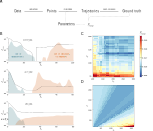
\includegraphics[width=1\textwidth]{part_1/assets/Figure_4.png}    
    \caption{\textbf{Optimisation des paramètres d'analyse basé sur $P_{swap}$} (\textbf{A}) Schéma du workflow d'optimisation : le résultat parfait de tracking est utilisée pour calculer $P_{swap}$ et créer une boucle de rétroaction sur les paramètres d'analyse. (\textbf{B}) $P_{swap}$ (noire) en fonction de la distance maximale $h_d$ (en pixels) pour trois films typiques. Les lignes verticales pour DRP\_001 indique que $P_{swap}$ descend à 0. Les distributions des déplacements entre deux images successives (bleue), et de distance aux voisins (orange) sont montrées pour comparaison. (\textbf{C}) $P_{swap}$ en fonction de la distance maximale $h_d$ et du temps de disparition maximal $h_t$ (en nombre d'images) pour PAR\_001 pour $s_d=95$ et $s_{\alpha}=60$. (\textbf{D}) $P_{swap}$ en fonction de la distance $s_d$ (en pixels) et de l'angle de normalisation $s_{\alpha}$ (en degrés) pour PAR\_001 avec $h_d=210$ et $h_t=90$. } 
    \label{part_1:fig_4}
    \end{figure}
	
	Une autre question souvent posée est de savoir avec quelle résolution temporelle acquérir le film. Une grande résolution permet de diminuer $P_{swap}$ et donc de réduire le post-traitement mais n'est pas toujours envisageable (limitation de la caméra, de l'illumination, nécessité d'un grand espace de stockage).
	Pour étudier l'impact de la fréquence d'enregistrement, on a sélectionné 7 films avec une bonne résolution temporelle et nous les avons dégradés pour à chaque fois calculer $P_{swap}$. Tracé en fonction du facteur de dégradation adimentionné $(f-f^{\star})\tau$, on voit que tous les $P_{swap}$ suivent une courbe maîtresse :
	$$
	    L(x)=\frac{1}{1+e^{-1}a}
	$$
	qui est une fonction logistique standard où $f^{\star}$ correspond au facteur de dégradation où $P_{swap}=0.5$, $\tau$ est un facteur de normalisation qui dépend des propriétés dynamiques de chaque système.
\medbreak
	
	A l'aide de ses résultats, on peut donc proposer une méthode permettant de déterminer la fréquence d'acquisition optimale. Cette méthode nécessite un seul enregistrement de bonne qualité déjà analysé avec FastTrack. Il faut ensuite répéter la procédure de dégradation et calculer le $P_{swap}$ résultant. Les $P_{swap}$ peuvent être ajustés à la fonction logistique pour en extraire les paramètres $f^{\star}$ et $\tau$. Il suffit ensuite de choisir la fréquence d'acquisition en fonction de la quantité de travail que l'utilisateur est prêt à fournir en post-traitement $N_{swap}=P_{swap}(N_{obj}-n_{ap})$.
	
	\begin{figure}[h]
    \centering
    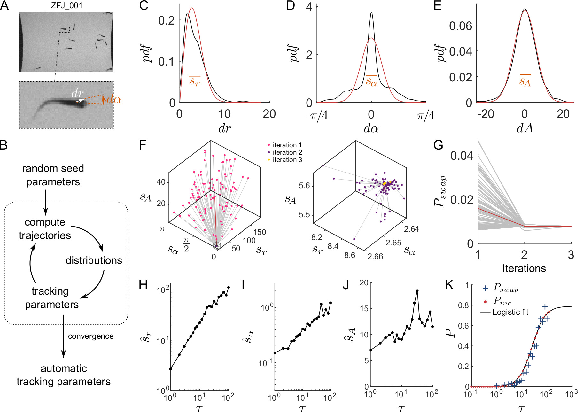
\includegraphics[width=1\textwidth]{part_1/assets/Figure_5.png}    
    \caption{\textbf{$P_{swap}$ et vitesse d’acquisition} (\textbf{A}) Schéma de la procédure de dégradation. (\textbf{B} $P_{swap}$ en fonction du taux réduit de dégradation $(f-f^{\star})\tau$ pour 7 systèmes très différents. $f^{\star}$ et $\tau$ ont été déterminés par un ajustement sur la fonction logistique standard (noire).}
    \label{part_1:fig_5}
    \end{figure}
	
\chapter{Perspective}

	On a vu dans cette partie le logiciel FastTrack. On a détaillé les outils utilisés ainsi que l'implémentation en elle-même. On a ensuite testé le logiciel sur une grande quantité de films présentant des systèmes extrêmement variés et évalué sa performance. On a décrit deux méthodes permettant de trouver facilement les paramètres optimaux d'analyses et la fréquence d'acquisition optimale qui permet de guider l'utilisateur de la conception de l'expérience jusqu'à l'analyse des films.
\medbreak
	
	Les codes du logiciel sont entièrement disponible à l'adresse \url{.}. Cela permet d'une part de collaborer au projet pour régler des bogues où ajouter des fonctionnalités. D'intégrer tout ou une partie du projet dans un logiciel ou une expérience déjà existante. Cela renforce la pérennité du projet qui ne dépend pas d'une seule personne pour rester à jour. Enfin la mise en place de la livraison continue (CD) permet de s'affranchir d'un temps dédié à la création de chaque version pour les trois plateformes supportées.
\medbreak
	
	La collaboration pour implémenter de nouvelles fonctionnalités, participer à la documentation ou régler des bogues est encouragée et peut se faire grâce au système de pull-request de GitHub.
	
	

